% Created by tikzDevice version 0.12.6 on 2025-07-14 15:46:10
% !TEX encoding = UTF-8 Unicode
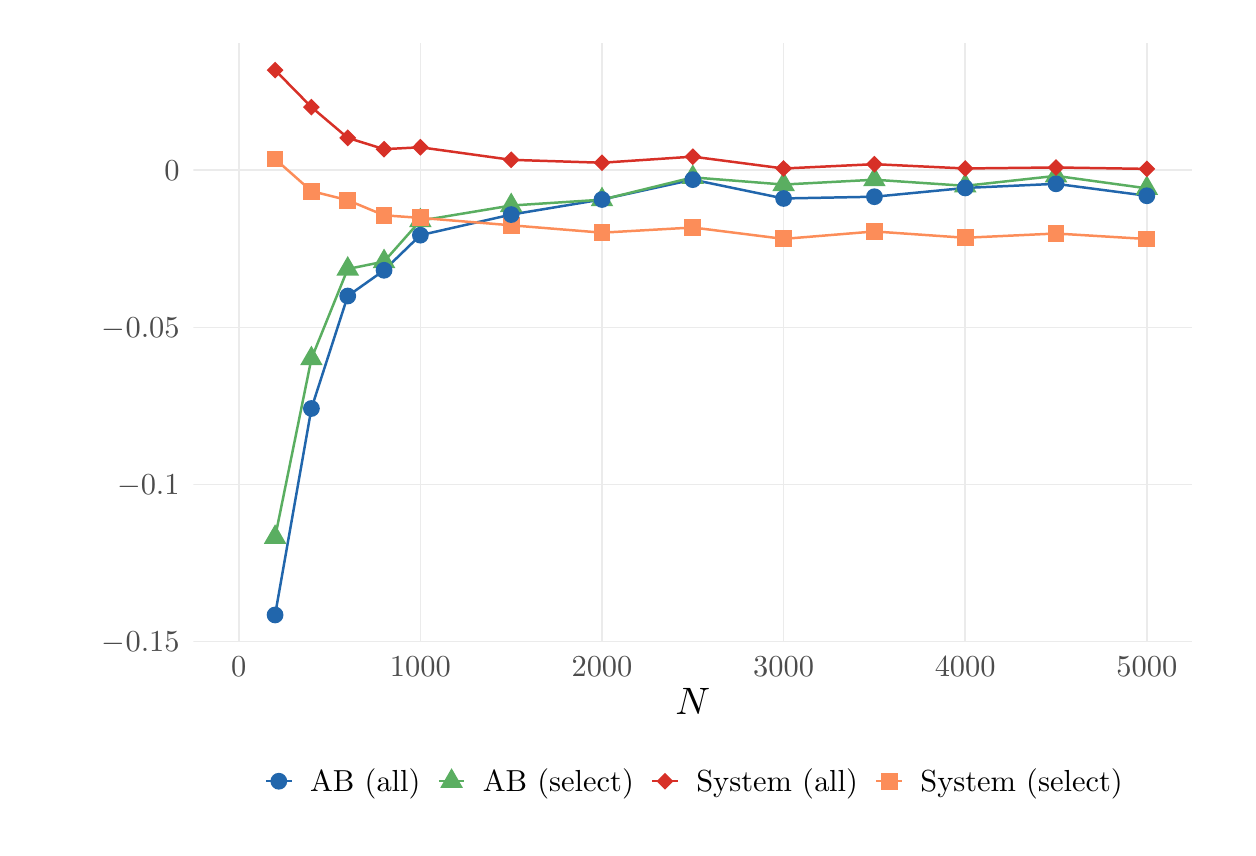
\begin{tikzpicture}[x=1pt,y=1pt]
\definecolor{fillColor}{RGB}{255,255,255}
\path[use as bounding box,fill=fillColor,fill opacity=0.00] (0,0) rectangle (433.62,289.08);
\begin{scope}
\path[clip] ( 59.87, 67.02) rectangle (420.81,283.58);
\definecolor{drawColor}{gray}{0.92}

\path[draw=drawColor,line width= 0.6pt,line join=round] ( 59.87, 67.33) --
	(420.81, 67.33);

\path[draw=drawColor,line width= 0.6pt,line join=round] ( 59.87,124.06) --
	(420.81,124.06);

\path[draw=drawColor,line width= 0.6pt,line join=round] ( 59.87,180.79) --
	(420.81,180.79);

\path[draw=drawColor,line width= 0.6pt,line join=round] ( 59.87,237.53) --
	(420.81,237.53);

\path[draw=drawColor,line width= 0.6pt,line join=round] ( 76.28, 67.02) --
	( 76.28,283.58);

\path[draw=drawColor,line width= 0.6pt,line join=round] (141.90, 67.02) --
	(141.90,283.58);

\path[draw=drawColor,line width= 0.6pt,line join=round] (207.53, 67.02) --
	(207.53,283.58);

\path[draw=drawColor,line width= 0.6pt,line join=round] (273.15, 67.02) --
	(273.15,283.58);

\path[draw=drawColor,line width= 0.6pt,line join=round] (338.78, 67.02) --
	(338.78,283.58);

\path[draw=drawColor,line width= 0.6pt,line join=round] (404.40, 67.02) --
	(404.40,283.58);
\definecolor{drawColor}{RGB}{33,102,172}

\path[draw=drawColor,line width= 0.9pt,line join=round] ( 89.40, 76.86) --
	(102.53,151.47) --
	(115.65,192.11) --
	(128.78,201.41) --
	(141.90,214.10) --
	(174.72,221.54) --
	(207.53,226.99) --
	(240.34,234.16) --
	(273.15,227.36) --
	(305.97,227.99) --
	(338.78,231.16) --
	(371.59,232.65) --
	(404.40,228.34);
\definecolor{drawColor}{RGB}{90,174,97}

\path[draw=drawColor,line width= 0.9pt,line join=round] ( 89.40,104.91) --
	(102.53,169.46) --
	(115.65,201.87) --
	(128.78,204.56) --
	(141.90,219.36) --
	(174.72,224.81) --
	(207.53,226.92) --
	(240.34,234.98) --
	(273.15,232.39) --
	(305.97,234.13) --
	(338.78,231.93) --
	(371.59,235.53) --
	(404.40,231.02);
\definecolor{drawColor}{RGB}{215,48,39}

\path[draw=drawColor,line width= 0.9pt,line join=round] ( 89.40,273.74) --
	(102.53,260.38) --
	(115.65,249.26) --
	(128.78,245.17) --
	(141.90,245.86) --
	(174.72,241.32) --
	(207.53,240.27) --
	(240.34,242.47) --
	(273.15,238.19) --
	(305.97,239.75) --
	(338.78,238.20) --
	(371.59,238.56) --
	(404.40,238.05);
\definecolor{drawColor}{RGB}{252,141,89}

\path[draw=drawColor,line width= 0.9pt,line join=round] ( 89.40,241.64) --
	(102.53,230.01) --
	(115.65,226.74) --
	(128.78,221.28) --
	(141.90,220.34) --
	(174.72,217.67) --
	(207.53,215.00) --
	(240.34,216.87) --
	(273.15,212.75) --
	(305.97,215.44) --
	(338.78,213.16) --
	(371.59,214.70) --
	(404.40,212.71);
\definecolor{fillColor}{RGB}{90,174,97}

\path[fill=fillColor] (141.90,224.08) --
	(145.99,217.00) --
	(137.82,217.00) --
	cycle;
\definecolor{fillColor}{RGB}{252,141,89}

\path[fill=fillColor] (138.87,217.31) --
	(144.94,217.31) --
	(144.94,223.38) --
	(138.87,223.38) --
	cycle;
\definecolor{fillColor}{RGB}{90,174,97}

\path[fill=fillColor] (174.72,229.52) --
	(178.80,222.45) --
	(170.63,222.45) --
	cycle;
\definecolor{fillColor}{RGB}{252,141,89}

\path[fill=fillColor] (171.68,214.63) --
	(177.75,214.63) --
	(177.75,220.70) --
	(171.68,220.70) --
	cycle;
\definecolor{fillColor}{RGB}{90,174,97}

\path[fill=fillColor] ( 89.40,109.63) --
	( 93.49,102.55) --
	( 85.32,102.55) --
	cycle;
\definecolor{fillColor}{RGB}{252,141,89}

\path[fill=fillColor] ( 86.37,238.61) --
	( 92.44,238.61) --
	( 92.44,244.67) --
	( 86.37,244.67) --
	cycle;
\definecolor{fillColor}{RGB}{90,174,97}

\path[fill=fillColor] (207.53,231.64) --
	(211.61,224.56) --
	(203.44,224.56) --
	cycle;
\definecolor{fillColor}{RGB}{252,141,89}

\path[fill=fillColor] (204.50,211.97) --
	(210.56,211.97) --
	(210.56,218.03) --
	(204.50,218.03) --
	cycle;
\definecolor{fillColor}{RGB}{90,174,97}

\path[fill=fillColor] (240.34,239.70) --
	(244.43,232.62) --
	(236.26,232.62) --
	cycle;
\definecolor{fillColor}{RGB}{252,141,89}

\path[fill=fillColor] (237.31,213.84) --
	(243.37,213.84) --
	(243.37,219.90) --
	(237.31,219.90) --
	cycle;
\definecolor{fillColor}{RGB}{90,174,97}

\path[fill=fillColor] (273.15,237.11) --
	(277.24,230.03) --
	(269.07,230.03) --
	cycle;
\definecolor{fillColor}{RGB}{252,141,89}

\path[fill=fillColor] (270.12,209.72) --
	(276.19,209.72) --
	(276.19,215.79) --
	(270.12,215.79) --
	cycle;
\definecolor{fillColor}{RGB}{90,174,97}

\path[fill=fillColor] (305.97,238.85) --
	(310.05,231.78) --
	(301.88,231.78) --
	cycle;
\definecolor{fillColor}{RGB}{252,141,89}

\path[fill=fillColor] (302.93,212.41) --
	(309.00,212.41) --
	(309.00,218.47) --
	(302.93,218.47) --
	cycle;
\definecolor{fillColor}{RGB}{90,174,97}

\path[fill=fillColor] (102.53,174.18) --
	(106.61,167.10) --
	( 98.44,167.10) --
	cycle;
\definecolor{fillColor}{RGB}{252,141,89}

\path[fill=fillColor] ( 99.50,226.98) --
	(105.56,226.98) --
	(105.56,233.05) --
	( 99.50,233.05) --
	cycle;
\definecolor{fillColor}{RGB}{90,174,97}

\path[fill=fillColor] (338.78,236.64) --
	(342.86,229.57) --
	(334.69,229.57) --
	cycle;
\definecolor{fillColor}{RGB}{252,141,89}

\path[fill=fillColor] (335.75,210.13) --
	(341.81,210.13) --
	(341.81,216.19) --
	(335.75,216.19) --
	cycle;
\definecolor{fillColor}{RGB}{90,174,97}

\path[fill=fillColor] (371.59,240.25) --
	(375.68,233.17) --
	(367.51,233.17) --
	cycle;
\definecolor{fillColor}{RGB}{252,141,89}

\path[fill=fillColor] (368.56,211.66) --
	(374.63,211.66) --
	(374.63,217.73) --
	(368.56,217.73) --
	cycle;
\definecolor{fillColor}{RGB}{90,174,97}

\path[fill=fillColor] (404.40,235.74) --
	(408.49,228.66) --
	(400.32,228.66) --
	cycle;
\definecolor{fillColor}{RGB}{252,141,89}

\path[fill=fillColor] (401.37,209.68) --
	(407.44,209.68) --
	(407.44,215.74) --
	(401.37,215.74) --
	cycle;
\definecolor{fillColor}{RGB}{90,174,97}

\path[fill=fillColor] (115.65,206.59) --
	(119.74,199.52) --
	(111.57,199.52) --
	cycle;
\definecolor{fillColor}{RGB}{252,141,89}

\path[fill=fillColor] (112.62,223.71) --
	(118.69,223.71) --
	(118.69,229.78) --
	(112.62,229.78) --
	cycle;
\definecolor{fillColor}{RGB}{90,174,97}

\path[fill=fillColor] (128.78,209.28) --
	(132.86,202.21) --
	(124.69,202.21) --
	cycle;
\definecolor{fillColor}{RGB}{252,141,89}

\path[fill=fillColor] (125.75,218.25) --
	(131.81,218.25) --
	(131.81,224.31) --
	(125.75,224.31) --
	cycle;
\definecolor{fillColor}{RGB}{33,102,172}

\path[fill=fillColor] (141.90,214.10) circle (  3.03);
\definecolor{fillColor}{RGB}{215,48,39}

\path[fill=fillColor] (138.87,245.86) --
	(141.90,248.90) --
	(144.94,245.86) --
	(141.90,242.83) --
	cycle;
\definecolor{fillColor}{RGB}{33,102,172}

\path[fill=fillColor] (174.72,221.54) circle (  3.03);
\definecolor{fillColor}{RGB}{215,48,39}

\path[fill=fillColor] (171.68,241.32) --
	(174.72,244.36) --
	(177.75,241.32) --
	(174.72,238.29) --
	cycle;
\definecolor{fillColor}{RGB}{33,102,172}

\path[fill=fillColor] ( 89.40, 76.86) circle (  3.03);
\definecolor{fillColor}{RGB}{215,48,39}

\path[fill=fillColor] ( 86.37,273.74) --
	( 89.40,276.77) --
	( 92.44,273.74) --
	( 89.40,270.70) --
	cycle;
\definecolor{fillColor}{RGB}{33,102,172}

\path[fill=fillColor] (207.53,226.99) circle (  3.03);
\definecolor{fillColor}{RGB}{215,48,39}

\path[fill=fillColor] (204.50,240.27) --
	(207.53,243.31) --
	(210.56,240.27) --
	(207.53,237.24) --
	cycle;
\definecolor{fillColor}{RGB}{33,102,172}

\path[fill=fillColor] (240.34,234.16) circle (  3.03);
\definecolor{fillColor}{RGB}{215,48,39}

\path[fill=fillColor] (237.31,242.47) --
	(240.34,245.50) --
	(243.37,242.47) --
	(240.34,239.43) --
	cycle;
\definecolor{fillColor}{RGB}{33,102,172}

\path[fill=fillColor] (273.15,227.36) circle (  3.03);
\definecolor{fillColor}{RGB}{215,48,39}

\path[fill=fillColor] (270.12,238.19) --
	(273.15,241.22) --
	(276.19,238.19) --
	(273.15,235.16) --
	cycle;
\definecolor{fillColor}{RGB}{33,102,172}

\path[fill=fillColor] (305.97,227.99) circle (  3.03);
\definecolor{fillColor}{RGB}{215,48,39}

\path[fill=fillColor] (302.93,239.75) --
	(305.97,242.78) --
	(309.00,239.75) --
	(305.97,236.71) --
	cycle;
\definecolor{fillColor}{RGB}{33,102,172}

\path[fill=fillColor] (102.53,151.47) circle (  3.03);
\definecolor{fillColor}{RGB}{215,48,39}

\path[fill=fillColor] ( 99.50,260.38) --
	(102.53,263.41) --
	(105.56,260.38) --
	(102.53,257.34) --
	cycle;
\definecolor{fillColor}{RGB}{33,102,172}

\path[fill=fillColor] (338.78,231.16) circle (  3.03);
\definecolor{fillColor}{RGB}{215,48,39}

\path[fill=fillColor] (335.75,238.20) --
	(338.78,241.23) --
	(341.81,238.20) --
	(338.78,235.17) --
	cycle;
\definecolor{fillColor}{RGB}{33,102,172}

\path[fill=fillColor] (371.59,232.65) circle (  3.03);
\definecolor{fillColor}{RGB}{215,48,39}

\path[fill=fillColor] (368.56,238.56) --
	(371.59,241.60) --
	(374.63,238.56) --
	(371.59,235.53) --
	cycle;
\definecolor{fillColor}{RGB}{33,102,172}

\path[fill=fillColor] (404.40,228.34) circle (  3.03);
\definecolor{fillColor}{RGB}{215,48,39}

\path[fill=fillColor] (401.37,238.05) --
	(404.40,241.09) --
	(407.44,238.05) --
	(404.40,235.02) --
	cycle;
\definecolor{fillColor}{RGB}{33,102,172}

\path[fill=fillColor] (115.65,192.11) circle (  3.03);
\definecolor{fillColor}{RGB}{215,48,39}

\path[fill=fillColor] (112.62,249.26) --
	(115.65,252.29) --
	(118.69,249.26) --
	(115.65,246.22) --
	cycle;
\definecolor{fillColor}{RGB}{33,102,172}

\path[fill=fillColor] (128.78,201.41) circle (  3.03);
\definecolor{fillColor}{RGB}{215,48,39}

\path[fill=fillColor] (125.75,245.17) --
	(128.78,248.21) --
	(131.81,245.17) --
	(128.78,242.14) --
	cycle;
\end{scope}
\begin{scope}
\path[clip] (  0.00,  0.00) rectangle (433.62,289.08);
\definecolor{drawColor}{gray}{0.30}

\node[text=drawColor,anchor=base east,inner sep=0pt, outer sep=0pt, scale=  1.10] at ( 54.92, 63.54) {$-0.15$};

\node[text=drawColor,anchor=base east,inner sep=0pt, outer sep=0pt, scale=  1.10] at ( 54.92,120.27) {$-0.1$};

\node[text=drawColor,anchor=base east,inner sep=0pt, outer sep=0pt, scale=  1.10] at ( 54.92,177.00) {$-0.05$};

\node[text=drawColor,anchor=base east,inner sep=0pt, outer sep=0pt, scale=  1.10] at ( 54.92,233.74) {$0$};
\end{scope}
\begin{scope}
\path[clip] (  0.00,  0.00) rectangle (433.62,289.08);
\definecolor{drawColor}{gray}{0.30}

\node[text=drawColor,anchor=base,inner sep=0pt, outer sep=0pt, scale=  1.10] at ( 76.28, 54.49) {$0$};

\node[text=drawColor,anchor=base,inner sep=0pt, outer sep=0pt, scale=  1.10] at (141.90, 54.49) {$1000$};

\node[text=drawColor,anchor=base,inner sep=0pt, outer sep=0pt, scale=  1.10] at (207.53, 54.49) {$2000$};

\node[text=drawColor,anchor=base,inner sep=0pt, outer sep=0pt, scale=  1.10] at (273.15, 54.49) {$3000$};

\node[text=drawColor,anchor=base,inner sep=0pt, outer sep=0pt, scale=  1.10] at (338.78, 54.49) {$4000$};

\node[text=drawColor,anchor=base,inner sep=0pt, outer sep=0pt, scale=  1.10] at (404.40, 54.49) {$5000$};
\end{scope}
\begin{scope}
\path[clip] (  0.00,  0.00) rectangle (433.62,289.08);
\definecolor{drawColor}{RGB}{0,0,0}

\node[text=drawColor,anchor=base,inner sep=0pt, outer sep=0pt, scale=  1.38] at (240.34, 40.85) {$N$};
\end{scope}
\begin{scope}
\path[clip] (  0.00,  0.00) rectangle (433.62,289.08);
\definecolor{drawColor}{RGB}{33,102,172}

\path[draw=drawColor,line width= 0.9pt,line join=round] ( 86.12, 16.78) -- ( 95.37, 16.78);
\end{scope}
\begin{scope}
\path[clip] (  0.00,  0.00) rectangle (433.62,289.08);
\definecolor{fillColor}{RGB}{33,102,172}

\path[fill=fillColor] ( 90.75, 16.78) circle (  3.03);
\end{scope}
\begin{scope}
\path[clip] (  0.00,  0.00) rectangle (433.62,289.08);
\definecolor{drawColor}{RGB}{90,174,97}

\path[draw=drawColor,line width= 0.9pt,line join=round] (148.55, 16.78) -- (157.80, 16.78);
\end{scope}
\begin{scope}
\path[clip] (  0.00,  0.00) rectangle (433.62,289.08);
\definecolor{fillColor}{RGB}{90,174,97}

\path[fill=fillColor] (153.18, 21.50) --
	(157.26, 14.42) --
	(149.09, 14.42) --
	cycle;
\end{scope}
\begin{scope}
\path[clip] (  0.00,  0.00) rectangle (433.62,289.08);
\definecolor{drawColor}{RGB}{215,48,39}

\path[draw=drawColor,line width= 0.9pt,line join=round] (225.71, 16.78) -- (234.96, 16.78);
\end{scope}
\begin{scope}
\path[clip] (  0.00,  0.00) rectangle (433.62,289.08);
\definecolor{fillColor}{RGB}{215,48,39}

\path[fill=fillColor] (227.30, 16.78) --
	(230.33, 19.81) --
	(233.36, 16.78) --
	(230.33, 13.75) --
	cycle;
\end{scope}
\begin{scope}
\path[clip] (  0.00,  0.00) rectangle (433.62,289.08);
\definecolor{drawColor}{RGB}{252,141,89}

\path[draw=drawColor,line width= 0.9pt,line join=round] (306.68, 16.78) -- (315.93, 16.78);
\end{scope}
\begin{scope}
\path[clip] (  0.00,  0.00) rectangle (433.62,289.08);
\definecolor{fillColor}{RGB}{252,141,89}

\path[fill=fillColor] (308.27, 13.75) --
	(314.34, 13.75) --
	(314.34, 19.81) --
	(308.27, 19.81) --
	cycle;
\end{scope}
\begin{scope}
\path[clip] (  0.00,  0.00) rectangle (433.62,289.08);
\definecolor{drawColor}{RGB}{0,0,0}

\node[text=drawColor,anchor=base west,inner sep=0pt, outer sep=0pt, scale=  1.10] at (102.03, 12.99) {AB (all)};
\end{scope}
\begin{scope}
\path[clip] (  0.00,  0.00) rectangle (433.62,289.08);
\definecolor{drawColor}{RGB}{0,0,0}

\node[text=drawColor,anchor=base west,inner sep=0pt, outer sep=0pt, scale=  1.10] at (164.46, 12.99) {AB (select)};
\end{scope}
\begin{scope}
\path[clip] (  0.00,  0.00) rectangle (433.62,289.08);
\definecolor{drawColor}{RGB}{0,0,0}

\node[text=drawColor,anchor=base west,inner sep=0pt, outer sep=0pt, scale=  1.10] at (241.61, 12.99) {System (all)};
\end{scope}
\begin{scope}
\path[clip] (  0.00,  0.00) rectangle (433.62,289.08);
\definecolor{drawColor}{RGB}{0,0,0}

\node[text=drawColor,anchor=base west,inner sep=0pt, outer sep=0pt, scale=  1.10] at (322.58, 12.99) {System (select)};
\end{scope}
\end{tikzpicture}
